\section{Linear Regression}

Regression should be a familiar topic. We will move quickly through what might be familiar and then introduce machine learning vocabulary and other points of emphasis. Some of this, like discussion of the loss surface, will feel unnecessary. However, this is a chance to ease into new concepts that will arise again for other prediction models.

\begin{readingbox}
\begin{itemize}
\item \cite{kuhn2013applied}, Chapter 6
\item \cite{hastie2009elements}, Chapter 3
\end{itemize}
\end{readingbox}

\subsection{OLS}

Can you think of some famous lines? Maybe you are thinking of the Equator, the Mason Dixon, or the line in the sand at the Alamo. We can do better. $\hat{y} = 68 + \frac{2}{3}(68-x)$ is the line from which we get the term \textbf{regression}.

\begin{displayquote}
``The height-deviate of the offspring is, on the average, two-thirds of the height-deviate of its mid-parentage.''\\
--- \cite{galton1886regression}
\end{displayquote}

Francis Galton found this line by observing that tall parents tended to have shorter (closer to average) children, while short parents tended to have taller kids. He described this phenomenon as ``regression to mediocrity,'' reflecting the tendency of extreme characteristics to move back toward the population average in subsequent generations. Galton actually used ``ocular regression'' (eyeballing it) and the term \textit{regression} has stuck for the general line-of-best-fit technique, even when applied to data that don't follow this pattern. Regression is also sometimes used to describe any kind of model that predicts a numeric value (for example, a decision tree might be called regression tree).

In 2025, ocular regression doesn't cut it. Ordinary least squares (OLS) is the most common method for estimating the parameters in a linear regression model. Linear models are flexible because they can still accommodate interactions, categorical predictors, and nonlinearities. You, the analyst, just have to include them in your specification.

Our predictors give us the design matrix, $X$. With $n$ observations and $k$ features (including an intercept), this is $n\times k$. The target variable is stored in the $n\times 1$ matrix, $y$.

Then, we find the regression coefficients $\hat{\beta}$, which might also be called the model \textbf{parameters}. Once the parameters are found, we can make predictions $X\hat{\beta}$ and $y-X \hat{\beta}$ is the vector of \textbf{residuals} or prediction errors.

\subsubsection{Optimization}

Parameters for any model are found by minimizing a \textbf{loss function} (also called a cost function\footnote{Cost and loss are used interchangeably but one might insist that the loss function is the individual function for each data point and the cost is the loss aggregated over all data points.}), which describes the quality of the model fit for particular parameter values. The parameters are found by minimizing the loss $L(\beta)$,

\begin{equation}
\hat{\beta} = \arg\min_{\beta} \left[ L(\beta) \right]
\label{eq:general-optimization}
\end{equation}

For least squares,

\begin{equation}
\hat{\beta} = \arg\min_{\beta} \sum_{i=1}^n (y_i - x_i^T\beta)^2
\label{eq:ols-optimization}
\end{equation}

$\hat{\beta}$ is simply where we find the minimum of $L(\beta)$ loss surface. The plot below illustrates such a surface for simple linear regression. Each point in the contour plot corresponds to an entirely different line of fit.

\begin{figure}[H]
\centering
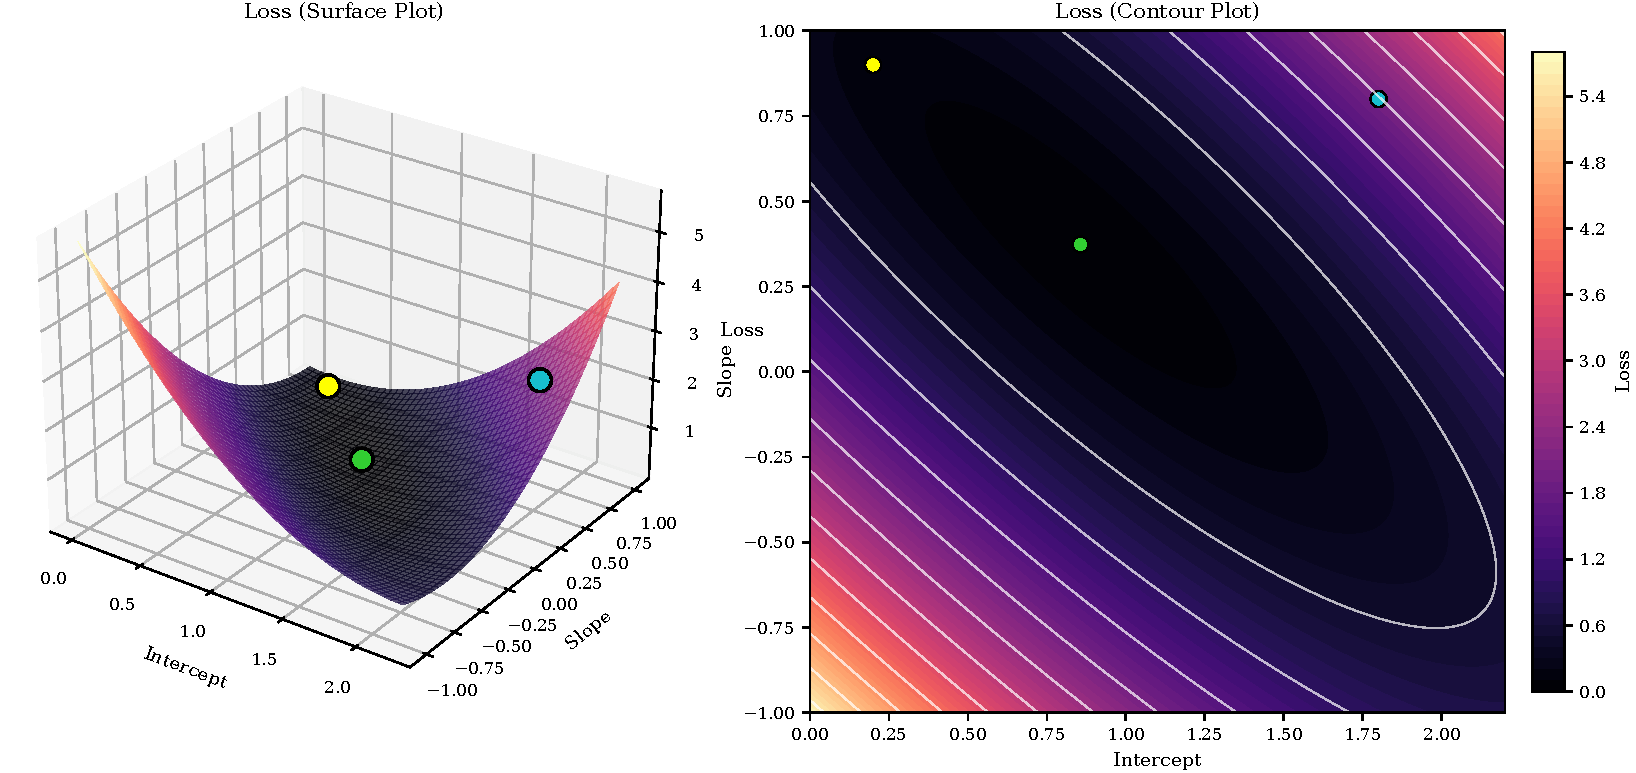
\includegraphics[width=\textwidth]{images/linear_reg_loss_surface.pdf}
\caption{Loss surface for simple linear regression showing 3D surface (left) and contour plot (right). Each point corresponds to different intercept and slope parameters. The minimum (green point) represents the OLS solution.}
\label{fig:loss-surface}
\end{figure}

The optimization is straightforward for OLS. The loss minimizing $\hat{\beta}$ is

\begin{equation}
\hat{\beta} = (X^TX)^{-1} X^T y
\label{eq:ols-solution}
\end{equation}

Because linear algebra is king in machine learning, we'll give the geometric interpretation. OLS solves a projection problem:

\begin{itemize}
\item The column space of $X$ is the set of all possible predictions we can make using linear combinations of our features. This forms a $k$-dimensional subspace in $\mathbb{R}^n$.
\item Our observed $y$ vector typically doesn't lie exactly in this column space (for example, for three points that you can't draw a single line through in simple linear regression).
\item OLS finds $\hat{\beta}$ such that $X\hat{\beta}$ is the vector of predictions in the column space closest to $y$.
\item $X\hat{\beta}$ is not the regression line. The regression line (or hyperplane) is the set of all points $(x_1, \dots ,x_{k-1}, x^T\hat{\beta})$.
\end{itemize}

Mathematically, $X\hat{\beta}$ is the orthogonal projection of $y$ onto the column space of $X$. Orthogonality is what makes $X\hat{\beta}$ closer to $y$ than any other candidate:

\begin{equation}
\Vert y - X\hat{\beta} \Vert \leq \Vert y - Xv \Vert
\label{eq:orthogonal-projection}
\end{equation}

for any other $k \times 1$ vector $v$. In other words, no other choice of coefficients can get us closer to $y$.

The quality of the fit is not generally measured by $\Vert y - X\hat{\beta} \Vert$.\footnote{$\Vert \cdot \Vert$ is the Euclidean or L2 norm.} Instead we usually report the mean squared error (MSE),

\begin{equation}
\mathrm{MSE} = \frac{1}{n} \sum_{i=1}^n (y_i - \hat{y}_i)^2 = \frac{1}{n}\Vert y - X\hat{\beta} \Vert^2
\label{eq:mse-linear}
\end{equation}

This scaling makes MSE comparable across datasets of different sizes.

\subsection{Regression Anatomy}

Multiple regression coefficients can be found as the slopes in a series of univariate regressions. 

Find the parameter $w_2$ from $\hat{y} = w_0 + w_1x_1 + w_2x_2$ by 

\begin{itemize}
\item Regress $x_2$ on $x_1$ (predict $x_2$ using $x_1$). Find the residuals $\tilde{x}_2$.

\item Find the residuals from prediciting $y$ from just $x_1$. 

\item Find $w_2$ by predicting the residuals from the second step using the residuals from the first. 

\end{itemize}

\subsection{Why OLS is special (two reasons)}

\textbf{Gauss Markov (BLUE).}
\begin{itemize}\itemsep0.2em
\item \emph{Claim.} Under the standard linear model conditions, the OLS estimator
$\hat\beta=(X^\top X)^{-1}X^\top y$ is the \emph{Best Linear Unbiased Estimator} (BLUE): among all linear unbiased estimators, it has the smallest variance.
\item \emph{Model setup.} $y = X\beta + \varepsilon$, with $X\in\mathbb{R}^{n\times k}$ (full column rank).
\item \emph{Sufficient conditions (with notation).}
  \begin{itemize}\itemsep0.15em
  \item \textbf{Linearity in parameters / correct specification:}
        $y = X\beta + \varepsilon$ (any nonlinear terms must appear as columns of $X$).
  \item \textbf{Exogeneity (zero conditional mean):}
        $\mathbb{E}[\varepsilon\mid X]=0$ \quad (equivalently $\mathbb{E}[X^\top\varepsilon]=0$ or $\mathrm{Cov}(X_j,\varepsilon)=0\ \forall j$).
  \item \textbf{Full rank (no exact multicollinearity):}
        $\mathrm{rank}(X)=k$ \ $\Rightarrow$ $X^\top X$ invertible.
  \item \textbf{Homoskedasticity (constant variance):}
        $\mathrm{Var}(\varepsilon_i\mid X)=\sigma^2$ for all $i$.
  \item \textbf{No autocorrelation (uncorrelated errors):}
        $\mathrm{Cov}(\varepsilon_i,\varepsilon_j\mid X)=0$ for $i\neq j$.
        \quad (Together with homoskedasticity: $\mathrm{Var}(\varepsilon\mid X)=\sigma^2 I_n$.)
  \end{itemize}
\end{itemize}

\textbf{OLS as Maximum Likelihood.}
\begin{itemize}\itemsep0.2em
\item \emph{Assumption.} $\varepsilon\mid X \stackrel{\text{i.i.d.}}{\sim} \mathcal{N}(0,\sigma^2)$.
\item \emph{Likelihood.} 
$L(\beta,\sigma^2\mid X,y)\propto (\sigma^2)^{-n/2}\exp\!\left(-\tfrac{1}{2\sigma^2}\|y-X\beta\|^2\right)$.
Maximizing over $\beta$ $\Longleftrightarrow$ minimizing $\sum_i (y_i-x_i^\top\beta)^2$, so the MLE of $\beta$ is OLS.
\end{itemize}



\subsection{Multicollinearity as Directional Instability}


When two predictors move together, changing their coefficients in opposite ways barely changes fitted values on the training data. Because squared loss cares about fitted values, the loss surface is \emph{flat} in those directions—so many different coefficient pairs fit almost equally well. That flatness is what makes coefficients unstable.


The following figure is based on a model where $y = x_1 + x_2 + \varepsilon$ so the true slopes are both one.  

\begin{figure}[H]
\centering
\begin{subfigure}[b]{0.32\textwidth}
    \centering
    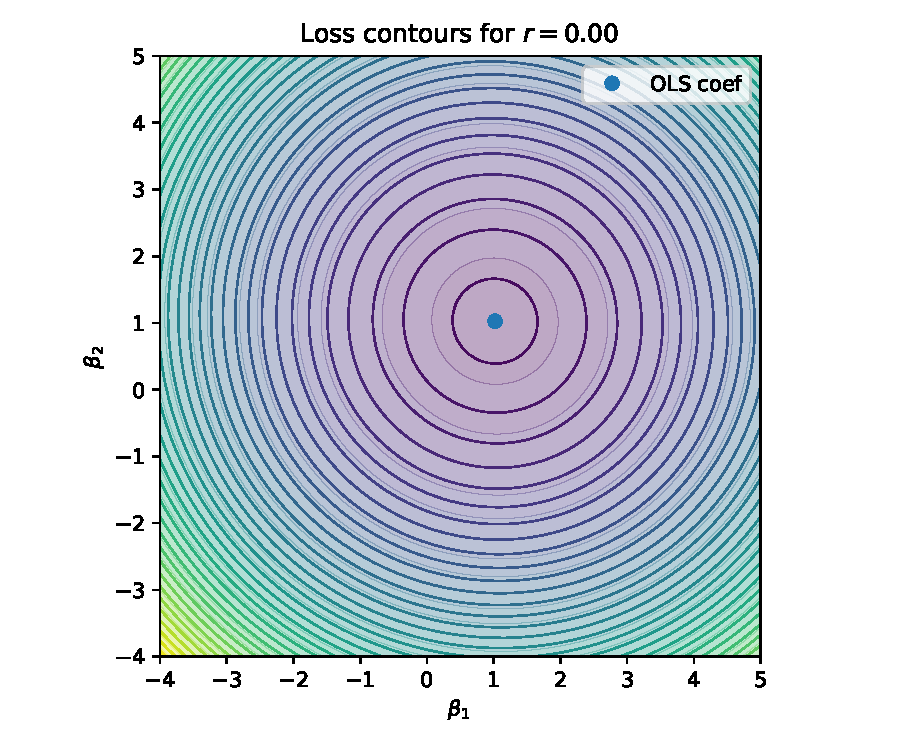
\includegraphics[width=\textwidth]{images/loss_contours_r0.pdf}
    \caption{$\rho = 0$}
    \label{fig:loss-contours-r0}
\end{subfigure}
\hfill
\begin{subfigure}[b]{0.32\textwidth}
    \centering
    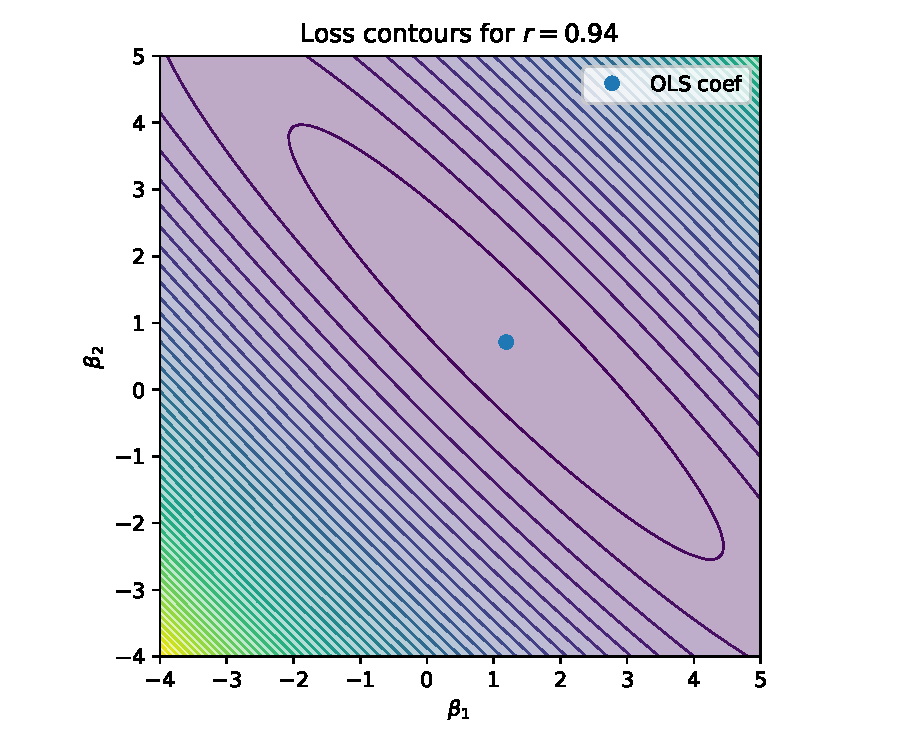
\includegraphics[width=\textwidth]{images/loss_contours_r94.pdf}
    \caption{$\rho = 0.94$}
    \label{fig:loss-contours-r94}
\end{subfigure}
\hfill
\begin{subfigure}[b]{0.32\textwidth}
    \centering
    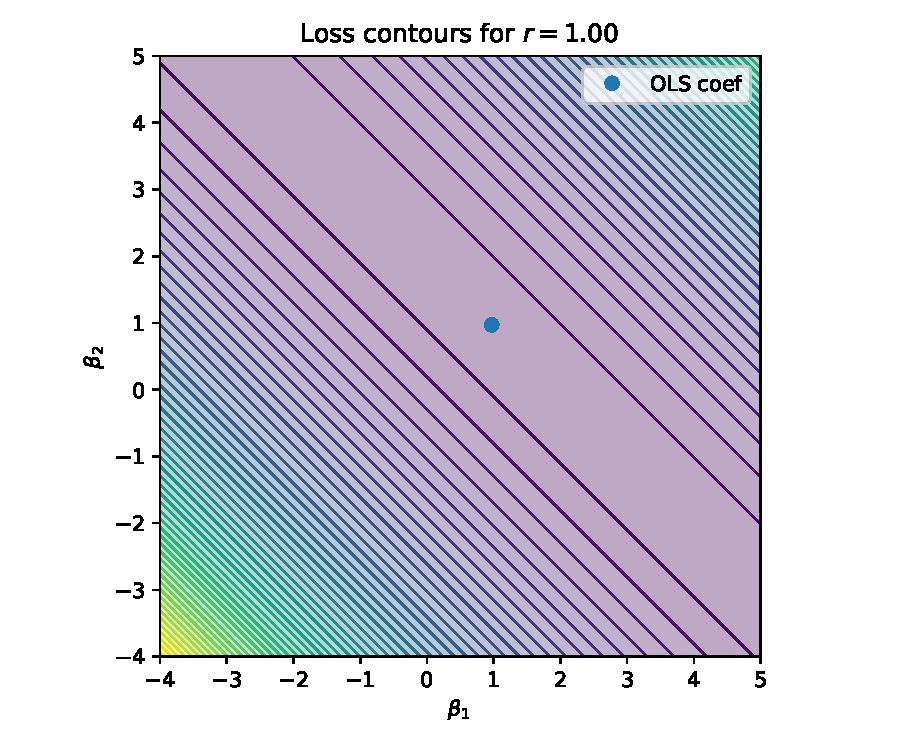
\includegraphics[width=\textwidth]{images/loss_contours_r100-1.pdf}
    \caption{$\rho \approx 1.0$}
    \label{fig:loss-contours-r100}
\end{subfigure}
\caption{Loss surface contours for two-feature linear regression with varying correlation $\rho$ between standardized features. Increasing correlation makes the loss surface more flat along the plane $x+y=2$, corresponding to increasing variance in the coefficients.}
\label{fig:loss-contours-correlation}
\end{figure}

The flatness of the loss surface creates more variance in the fitted coefficients.

\begin{figure}[H]
\centering
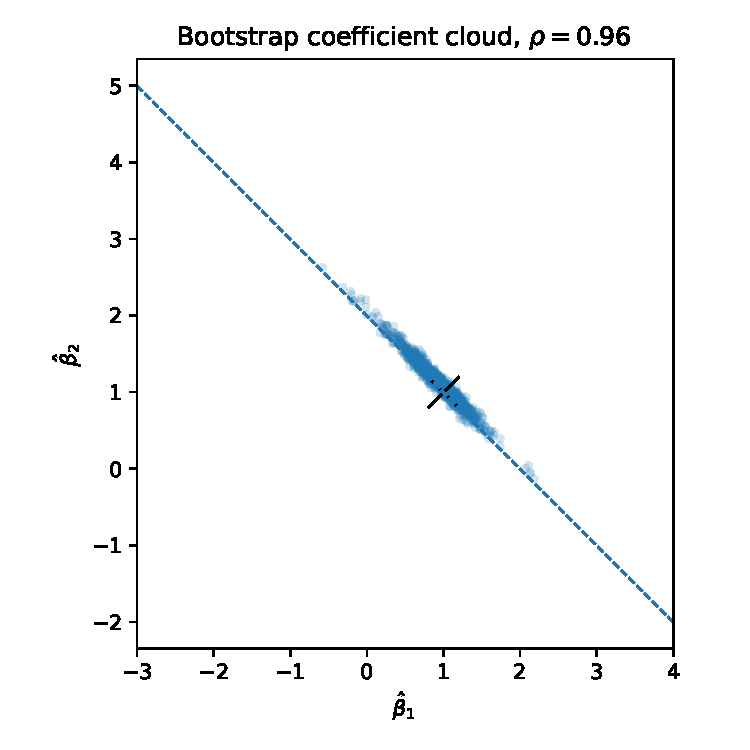
\includegraphics[width=.5\textwidth]{images/bootstrap_coef_cloud.pdf}
\end{figure}



\paragraph{What this means in practice.}
\begin{itemize}\itemsep0.2em
\item \textbf{Coefficient instability.} Because the loss barely changes in the ``swap'' direction, small data perturbations can swing $\hat\beta_1$ up and $\hat\beta_2$ down (or vice‑versa) with almost no change in training error—producing sign flips and large reported standard errors.
\item \textbf{In‑sample predictions can still look fine.} Many different coefficient pairs give nearly the same $\hat y$ when $x_1\approx x_2$. The instability is about \emph{coefficients}, not necessarily about in‑sample fit.
\item \textbf{Out‑of‑sample risk.} Predictions are fragile when a new case has $x_{*1}$ and $x_{*2}$ pulling in opposite ways (large $x_{*1}-x_{*2}$). That’s precisely the direction your training data did not pin down well.
\item \textbf{Quick checks.} Inspect the correlation matrix (or VIFs) and plot $x_1$ vs.\ $x_2$. Compositional features (shares summing to one) and poorly chosen reference categories are common sources—reparameterize to remove exact or near‑exact duplicates.
\end{itemize}




\subsection{Feature Engineering}

Once you have fixed the set of predictor variables (and thus the design matrix $X$), there is no \textbf{tuning} to do for OLS. The important choice for OLS is what variables (or transformations of variables) to include. The process of refining your set of predictor variables (features) is called \textbf{feature engineering}.

You should already be familiar with feature engineering, if not by that name. Review \cite{kuhn2013applied} Chapter 3 for an overview of variable transformations. Let's cover a few.

\subsubsection{Standardization}

Standardization (also called z-score normalization) transforms features to have mean 0 and standard deviation 1:

\begin{equation}
x_{\text{standardized}} = \frac{x - \mu}{\sigma}
\label{eq:standardization}
\end{equation}

This is particularly important when features have different scales (e.g., age in years vs income in dollars).

\subsubsection{Normalization}

Min-max normalization scales features to a fixed range, typically [0,1]:

\begin{equation}
x_{\text{normalized}} = \frac{x - x_{\min}}{x_{\max} - x_{\min}}
\label{eq:normalization}
\end{equation}

\subsubsection{One-hot Encoding}

For categorical variables, one-hot encoding creates binary indicator variables for each category. A categorical variable with $k$ levels becomes $k-1$ binary variables (to avoid the dummy variable trap).

\subsubsection{Principal Components}

Principal Component Analysis (PCA) creates new features that are linear combinations of the original features, ordered by how much variance they explain in the data. This can be useful for dimensionality reduction and handling multicollinearity.